% Options for packages loaded elsewhere
% Options for packages loaded elsewhere
\PassOptionsToPackage{unicode}{hyperref}
\PassOptionsToPackage{hyphens}{url}
\PassOptionsToPackage{dvipsnames,svgnames,x11names}{xcolor}
%
\documentclass[
  letterpaper,
  DIV=11,
  numbers=noendperiod]{scrartcl}
\usepackage{xcolor}
\usepackage{amsmath,amssymb}
\setcounter{secnumdepth}{5}
\usepackage{iftex}
\ifPDFTeX
  \usepackage[T1]{fontenc}
  \usepackage[utf8]{inputenc}
  \usepackage{textcomp} % provide euro and other symbols
\else % if luatex or xetex
  \usepackage{unicode-math} % this also loads fontspec
  \defaultfontfeatures{Scale=MatchLowercase}
  \defaultfontfeatures[\rmfamily]{Ligatures=TeX,Scale=1}
\fi
\usepackage{lmodern}
\ifPDFTeX\else
  % xetex/luatex font selection
\fi
% Use upquote if available, for straight quotes in verbatim environments
\IfFileExists{upquote.sty}{\usepackage{upquote}}{}
\IfFileExists{microtype.sty}{% use microtype if available
  \usepackage[]{microtype}
  \UseMicrotypeSet[protrusion]{basicmath} % disable protrusion for tt fonts
}{}
\makeatletter
\@ifundefined{KOMAClassName}{% if non-KOMA class
  \IfFileExists{parskip.sty}{%
    \usepackage{parskip}
  }{% else
    \setlength{\parindent}{0pt}
    \setlength{\parskip}{6pt plus 2pt minus 1pt}}
}{% if KOMA class
  \KOMAoptions{parskip=half}}
\makeatother
% Make \paragraph and \subparagraph free-standing
\makeatletter
\ifx\paragraph\undefined\else
  \let\oldparagraph\paragraph
  \renewcommand{\paragraph}{
    \@ifstar
      \xxxParagraphStar
      \xxxParagraphNoStar
  }
  \newcommand{\xxxParagraphStar}[1]{\oldparagraph*{#1}\mbox{}}
  \newcommand{\xxxParagraphNoStar}[1]{\oldparagraph{#1}\mbox{}}
\fi
\ifx\subparagraph\undefined\else
  \let\oldsubparagraph\subparagraph
  \renewcommand{\subparagraph}{
    \@ifstar
      \xxxSubParagraphStar
      \xxxSubParagraphNoStar
  }
  \newcommand{\xxxSubParagraphStar}[1]{\oldsubparagraph*{#1}\mbox{}}
  \newcommand{\xxxSubParagraphNoStar}[1]{\oldsubparagraph{#1}\mbox{}}
\fi
\makeatother

\usepackage{color}
\usepackage{fancyvrb}
\newcommand{\VerbBar}{|}
\newcommand{\VERB}{\Verb[commandchars=\\\{\}]}
\DefineVerbatimEnvironment{Highlighting}{Verbatim}{commandchars=\\\{\}}
% Add ',fontsize=\small' for more characters per line
\usepackage{framed}
\definecolor{shadecolor}{RGB}{241,243,245}
\newenvironment{Shaded}{\begin{snugshade}}{\end{snugshade}}
\newcommand{\AlertTok}[1]{\textcolor[rgb]{0.68,0.00,0.00}{#1}}
\newcommand{\AnnotationTok}[1]{\textcolor[rgb]{0.37,0.37,0.37}{#1}}
\newcommand{\AttributeTok}[1]{\textcolor[rgb]{0.40,0.45,0.13}{#1}}
\newcommand{\BaseNTok}[1]{\textcolor[rgb]{0.68,0.00,0.00}{#1}}
\newcommand{\BuiltInTok}[1]{\textcolor[rgb]{0.00,0.23,0.31}{#1}}
\newcommand{\CharTok}[1]{\textcolor[rgb]{0.13,0.47,0.30}{#1}}
\newcommand{\CommentTok}[1]{\textcolor[rgb]{0.37,0.37,0.37}{#1}}
\newcommand{\CommentVarTok}[1]{\textcolor[rgb]{0.37,0.37,0.37}{\textit{#1}}}
\newcommand{\ConstantTok}[1]{\textcolor[rgb]{0.56,0.35,0.01}{#1}}
\newcommand{\ControlFlowTok}[1]{\textcolor[rgb]{0.00,0.23,0.31}{\textbf{#1}}}
\newcommand{\DataTypeTok}[1]{\textcolor[rgb]{0.68,0.00,0.00}{#1}}
\newcommand{\DecValTok}[1]{\textcolor[rgb]{0.68,0.00,0.00}{#1}}
\newcommand{\DocumentationTok}[1]{\textcolor[rgb]{0.37,0.37,0.37}{\textit{#1}}}
\newcommand{\ErrorTok}[1]{\textcolor[rgb]{0.68,0.00,0.00}{#1}}
\newcommand{\ExtensionTok}[1]{\textcolor[rgb]{0.00,0.23,0.31}{#1}}
\newcommand{\FloatTok}[1]{\textcolor[rgb]{0.68,0.00,0.00}{#1}}
\newcommand{\FunctionTok}[1]{\textcolor[rgb]{0.28,0.35,0.67}{#1}}
\newcommand{\ImportTok}[1]{\textcolor[rgb]{0.00,0.46,0.62}{#1}}
\newcommand{\InformationTok}[1]{\textcolor[rgb]{0.37,0.37,0.37}{#1}}
\newcommand{\KeywordTok}[1]{\textcolor[rgb]{0.00,0.23,0.31}{\textbf{#1}}}
\newcommand{\NormalTok}[1]{\textcolor[rgb]{0.00,0.23,0.31}{#1}}
\newcommand{\OperatorTok}[1]{\textcolor[rgb]{0.37,0.37,0.37}{#1}}
\newcommand{\OtherTok}[1]{\textcolor[rgb]{0.00,0.23,0.31}{#1}}
\newcommand{\PreprocessorTok}[1]{\textcolor[rgb]{0.68,0.00,0.00}{#1}}
\newcommand{\RegionMarkerTok}[1]{\textcolor[rgb]{0.00,0.23,0.31}{#1}}
\newcommand{\SpecialCharTok}[1]{\textcolor[rgb]{0.37,0.37,0.37}{#1}}
\newcommand{\SpecialStringTok}[1]{\textcolor[rgb]{0.13,0.47,0.30}{#1}}
\newcommand{\StringTok}[1]{\textcolor[rgb]{0.13,0.47,0.30}{#1}}
\newcommand{\VariableTok}[1]{\textcolor[rgb]{0.07,0.07,0.07}{#1}}
\newcommand{\VerbatimStringTok}[1]{\textcolor[rgb]{0.13,0.47,0.30}{#1}}
\newcommand{\WarningTok}[1]{\textcolor[rgb]{0.37,0.37,0.37}{\textit{#1}}}

\usepackage{longtable,booktabs,array}
\newcounter{none} % for unnumbered tables
\usepackage{calc} % for calculating minipage widths
% Correct order of tables after \paragraph or \subparagraph
\usepackage{etoolbox}
\makeatletter
\patchcmd\longtable{\par}{\if@noskipsec\mbox{}\fi\par}{}{}
\makeatother
% Allow footnotes in longtable head/foot
\IfFileExists{footnotehyper.sty}{\usepackage{footnotehyper}}{\usepackage{footnote}}
\makesavenoteenv{longtable}
\usepackage{graphicx}
\makeatletter
\newsavebox\pandoc@box
\newcommand*\pandocbounded[1]{% scales image to fit in text height/width
  \sbox\pandoc@box{#1}%
  \Gscale@div\@tempa{\textheight}{\dimexpr\ht\pandoc@box+\dp\pandoc@box\relax}%
  \Gscale@div\@tempb{\linewidth}{\wd\pandoc@box}%
  \ifdim\@tempb\p@<\@tempa\p@\let\@tempa\@tempb\fi% select the smaller of both
  \ifdim\@tempa\p@<\p@\scalebox{\@tempa}{\usebox\pandoc@box}%
  \else\usebox{\pandoc@box}%
  \fi%
}
% Set default figure placement to htbp
\def\fps@figure{htbp}
\makeatother





\setlength{\emergencystretch}{3em} % prevent overfull lines

\providecommand{\tightlist}{%
  \setlength{\itemsep}{0pt}\setlength{\parskip}{0pt}}



 


\KOMAoption{captions}{tableheading}
\makeatletter
\@ifpackageloaded{caption}{}{\usepackage{caption}}
\AtBeginDocument{%
\ifdefined\contentsname
  \renewcommand*\contentsname{Table of contents}
\else
  \newcommand\contentsname{Table of contents}
\fi
\ifdefined\listfigurename
  \renewcommand*\listfigurename{List of Figures}
\else
  \newcommand\listfigurename{List of Figures}
\fi
\ifdefined\listtablename
  \renewcommand*\listtablename{List of Tables}
\else
  \newcommand\listtablename{List of Tables}
\fi
\ifdefined\figurename
  \renewcommand*\figurename{Figure}
\else
  \newcommand\figurename{Figure}
\fi
\ifdefined\tablename
  \renewcommand*\tablename{Table}
\else
  \newcommand\tablename{Table}
\fi
}
\@ifpackageloaded{float}{}{\usepackage{float}}
\floatstyle{ruled}
\@ifundefined{c@chapter}{\newfloat{codelisting}{h}{lop}}{\newfloat{codelisting}{h}{lop}[chapter]}
\floatname{codelisting}{Listing}
\newcommand*\listoflistings{\listof{codelisting}{List of Listings}}
\makeatother
\makeatletter
\makeatother
\makeatletter
\@ifpackageloaded{caption}{}{\usepackage{caption}}
\@ifpackageloaded{subcaption}{}{\usepackage{subcaption}}
\makeatother
\usepackage{bookmark}
\IfFileExists{xurl.sty}{\usepackage{xurl}}{} % add URL line breaks if available
\urlstyle{same}
\hypersetup{
  pdftitle={Three-Way Equity Classifier Comparison},
  pdfauthor={Group 8 \textbar{} University of South Florida},
  colorlinks=true,
  linkcolor={blue},
  filecolor={Maroon},
  citecolor={Blue},
  urlcolor={Blue},
  pdfcreator={LaTeX via pandoc}}


\title{Three-Way Equity Classifier Comparison}
\usepackage{etoolbox}
\makeatletter
\providecommand{\subtitle}[1]{% add subtitle to \maketitle
  \apptocmd{\@title}{\par {\large #1 \par}}{}{}
}
\makeatother
\subtitle{GICS Sectors vs.~SIC/FF12 Industries vs.~K-Means Co-Movement
Clusters}
\author{Group 8 \textbar{} University of South Florida}
\date{2026-04-27}
\begin{document}
\maketitle

\renewcommand*\contentsname{Table of contents}
{
\setcounter{tocdepth}{3}
\tableofcontents
}

\section{Executive summary}\label{executive-summary}

This project asks whether data-driven groupings of S\&P 500 stocks
classify firms more coherently than the GICS industry standard, and
whether one grouping scheme produces better return-anomaly signals than
another. We compare three classification systems head-to-head:

\begin{enumerate}
\def\labelenumi{\arabic{enumi}.}
\tightlist
\item
  \textbf{GICS sectors} --- the eleven Global Industry Classification
  Standard sectors that the index providers use.
\item
  \textbf{SIC-based FF12 industries} --- Ken French's twelve-industry
  partition, which is built directly from SIC codes and is the
  academic-finance counterpart to GICS.
\item
  \textbf{K-Means clusters on return co-movement} --- an unsupervised
  partition that groups stocks whose monthly excess returns move
  together over a rolling sixty-month window, refit annually with label
  matching.
\end{enumerate}

All three schemes are fed through the same downstream pipeline on the
same data, and we compare them on four dimensions: composition overlap,
within-group homogeneity, predictive accuracy on one-month-forward
alpha, and anomaly-detection behaviour.

Two design choices, made in response to feedback on an earlier draft of
this project, deserve to be flagged at the top:

\begin{itemize}
\tightlist
\item
  \textbf{The target is alpha, not raw return.} Predicting realised
  return from factor exposures would mostly recover the standard risk
  premia (high-beta stocks earn higher returns on average) --- a
  tautology, not a finding. The economically interesting quantity is the
  residual after factor exposure is priced out, i.e.~realised alpha. We
  predict \(\alpha_{i,t+1}\) throughout.
\item
  \textbf{FF factors enter as features only with a publication lag.} Ken
  French's data library publishes FF5 with a multi-month delay, so a
  forecast that consumes contemporaneous FF values would be unusable in
  real time. Every feature derived from FF returns is lagged by 2
  months. (Realised alpha at month \(t\) is computed from \(F_t\), but
  it is a \emph{label} --- never a feature input --- so this is
  internally consistent.)
\end{itemize}

The dataset and pipeline are built with the dev-mode toggle in
\texttt{CFG}. The HTML version of this report renders to the full S\&P
500 universe when \texttt{CFG\$dev\_mode\ =\ FALSE}; we leave dev mode
on here for reproducibility on modest hardware. Numbers and figures will
tighten when run on the full universe.

\section{1. Research question}\label{research-question}

Do data-driven groupings of S\&P 500 stocks classify firms more
coherently than GICS sectors, and do they better surface forward-alpha
anomalies?

This restates the question we posed in the original project blueprint in
two ways. First, we no longer compare an industry classification (GICS)
to a \emph{risk} taxonomy (FF5 loadings), because those are
incommensurable. The right comparison set for an industry classification
is other industry classifications --- GICS, SIC/FF12, and an
unsupervised industry-style clustering. Second, we judge ``better
classification'' not just on predictive R² but also on within-group
homogeneity (do members really behave alike?) and on anomaly-flagging
quality (do flagged outliers subsequently earn different forward
alpha?).

\section{2. Methods}\label{methods}

\subsection{2.1 The three classification
schemes}\label{the-three-classification-schemes}

\textbf{GICS sectors.} Eleven sectors assigned per stock-month via the
CRSP/Compustat Merged (CCM) linkage. Membership is point-in-time: a
stock that switches sectors mid-sample carries the new sector going
forward.

\textbf{SIC/FF12.} Each stock-month's SIC code (from CRSP
\texttt{stocknames}, respecting historical name ranges) is mapped to one
of twelve Ken French industries. SIC codes that fall outside any range
get assigned to ``Other.''

\textbf{K-Means clusters on return co-movement.} At the end of each
calendar year, we take the prior sixty months of monthly excess returns.
For each stock with at least thirty-six valid months we form a feature
vector equal to that stock's column of the cross-sectional correlation
matrix --- i.e.~each stock is described by its correlation with every
other stock in the panel. We reduce to ten principal components and fit
K-Means for \(k \in \{2, \ldots, 10\}\), picking \(k\) that maximises
the mean silhouette. The fitted assignment is used for all twelve months
of the following calendar year. Cluster identities are kept stable
across refits by Hungarian-algorithm matching against the previous fit's
labels.

\subsection{2.2 Target: realised alpha}\label{target-realised-alpha}

For each stock-month we compute realised alpha as the residual from the
five-factor model: \[
\alpha_{i,t} \;=\; r^e_{i,t} \;-\; \sum_{k \in \{\text{Mkt},\text{SMB},\text{HML},\text{RMW},\text{CMA}\}} \hat\beta_{i,k}\, F_{k,t},
\] where \(r^e_{i,t}\) is excess return and \(\hat\beta_{i,k}\) is
estimated by OLS on the 36-month window ending at month \(t-2\). The
forward target used throughout is \(\alpha_{i,t+1}\) --- realised alpha
one month ahead --- attached to the row at month \(t\).

\subsection{2.3 Features}\label{features}

The feature vector at month \(t\) contains:

\begin{itemize}
\tightlist
\item
  Cross-sectionally z-scored FF5 betas (\texttt{z\_beta\_*}), ranking
  each stock against the cross-section at the same date.
\item
  12-1 momentum (cumulative return from \(t-12\) to \(t-2\)), 12-month
  vol of excess returns, and log market cap lagged one month.
\item
  Lagged macro: 10-year Treasury yield, Fed funds rate, VIX --- each
  lagged one month.
\item
  Lagged FF5 returns (\texttt{mkt\_rf\_lag}, \texttt{smb\_lag},
  \texttt{hml\_lag}, \texttt{rmw\_lag}, \texttt{cma\_lag}) --- each
  lagged 2 months to honour the publication delay.
\end{itemize}

\subsection{2.4 Evaluation}\label{evaluation}

Train: January 2018 -- December 2022 (after the 36-month rolling-beta
warm-up consumes 2014--2017). Holdout: January 2023 -- December 2024.
All metrics report on the holdout.

\section{3. Data assembly}\label{data-assembly}

\subsection{3.1 Pull CRSP}\label{pull-crsp}

Historical S\&P 500 membership, monthly returns adjusted for delisting,
historical SIC codes, and GICS via the CCM linkage.

\begin{Shaded}
\begin{Highlighting}[]
\NormalTok{crsp }\OtherTok{\textless{}{-}} \FunctionTok{pull\_crsp\_all}\NormalTok{()}
\end{Highlighting}
\end{Shaded}

\begin{verbatim}
[18:29:10] Pulling Compustat data from 2014-01-01 to 2024-12-31
[18:29:10] cache hit:  data/raw/sp500_members.parquet
[18:29:10] cache hit:  data/raw/crsp_msf.parquet
[18:29:10] cache hit:  data/raw/crsp_stocknames.parquet
[18:29:10] cache hit:  data/raw/crsp_sic_history.parquet
[18:29:10] cache hit:  data/raw/ccm_gics.parquet
\end{verbatim}

\begin{Shaded}
\begin{Highlighting}[]
\NormalTok{crsp}\SpecialCharTok{$}\NormalTok{members }\SpecialCharTok{|\textgreater{}}
  \FunctionTok{summarise}\NormalTok{(}
    \AttributeTok{spans =} \FunctionTok{n}\NormalTok{(),}
    \AttributeTok{permnos =} \FunctionTok{n\_distinct}\NormalTok{(permno),}
    \AttributeTok{earliest\_start =} \FunctionTok{min}\NormalTok{(start),}
    \AttributeTok{latest\_end =} \FunctionTok{max}\NormalTok{(end\_date)}
\NormalTok{  ) }\SpecialCharTok{|\textgreater{}}
  \FunctionTok{kable}\NormalTok{(}\AttributeTok{caption =} \StringTok{"S\&P 500 membership spans"}\NormalTok{)}
\end{Highlighting}
\end{Shaded}

\begin{longtable}[]{@{}rrll@{}}
\caption{S\&P 500 membership spans}\tabularnewline
\toprule\noalign{}
spans & permnos & earliest\_start & latest\_end \\
\midrule\noalign{}
\endfirsthead
\toprule\noalign{}
spans & permnos & earliest\_start & latest\_end \\
\midrule\noalign{}
\endhead
\bottomrule\noalign{}
\endlastfoot
476 & 476 & 1964-03-31 & 2024-12-31 \\
\end{longtable}

\begin{Shaded}
\begin{Highlighting}[]
\NormalTok{crsp}\SpecialCharTok{$}\NormalTok{monthly }\SpecialCharTok{|\textgreater{}}
  \FunctionTok{summarise}\NormalTok{(}
    \AttributeTok{rows =} \FunctionTok{n}\NormalTok{(),}
    \AttributeTok{permnos =} \FunctionTok{n\_distinct}\NormalTok{(permno),}
    \AttributeTok{months =} \FunctionTok{n\_distinct}\NormalTok{(date\_eom),}
    \AttributeTok{delisting\_obs =} \FunctionTok{sum}\NormalTok{(}\SpecialCharTok{!}\FunctionTok{is.na}\NormalTok{(dlret)),}
    \AttributeTok{pct\_ret\_present =} \FunctionTok{mean}\NormalTok{(}\SpecialCharTok{!}\FunctionTok{is.na}\NormalTok{(ret))}
\NormalTok{  ) }\SpecialCharTok{|\textgreater{}}
  \FunctionTok{kable}\NormalTok{(}\AttributeTok{digits =} \DecValTok{3}\NormalTok{, }\AttributeTok{caption =} \StringTok{"Monthly return panel"}\NormalTok{)}
\end{Highlighting}
\end{Shaded}

\begin{longtable}[]{@{}rrrrr@{}}
\caption{Monthly return panel}\tabularnewline
\toprule\noalign{}
rows & permnos & months & delisting\_obs & pct\_ret\_present \\
\midrule\noalign{}
\endfirsthead
\toprule\noalign{}
rows & permnos & months & delisting\_obs & pct\_ret\_present \\
\midrule\noalign{}
\endhead
\bottomrule\noalign{}
\endlastfoot
62907 & 498 & 132 & 0 & 0.999 \\
\end{longtable}

\subsection{3.2 Pull Ken French}\label{pull-ken-french}

\begin{Shaded}
\begin{Highlighting}[]
\NormalTok{french }\OtherTok{\textless{}{-}} \FunctionTok{pull\_french\_all}\NormalTok{()}
\end{Highlighting}
\end{Shaded}

\begin{verbatim}
[18:29:10] Pulling Ken French data
[18:29:10] cache hit:  data/raw/ff5.parquet
[18:29:10] cache hit:  data/raw/ff12_def.parquet
\end{verbatim}

\begin{Shaded}
\begin{Highlighting}[]
\FunctionTok{bind\_rows}\NormalTok{(}\FunctionTok{head}\NormalTok{(french}\SpecialCharTok{$}\NormalTok{ff5, }\DecValTok{3}\NormalTok{), }\FunctionTok{tail}\NormalTok{(french}\SpecialCharTok{$}\NormalTok{ff5, }\DecValTok{3}\NormalTok{)) }\SpecialCharTok{|\textgreater{}}
  \FunctionTok{kable}\NormalTok{(}\AttributeTok{digits =} \DecValTok{4}\NormalTok{, }\AttributeTok{caption =} \StringTok{"FF5 factors — head and tail"}\NormalTok{)}
\end{Highlighting}
\end{Shaded}

\begin{longtable}[]{@{}lrrrrrr@{}}
\caption{FF5 factors --- head and tail}\tabularnewline
\toprule\noalign{}
date\_eom & mkt\_rf & smb & hml & rmw & cma & rf \\
\midrule\noalign{}
\endfirsthead
\toprule\noalign{}
date\_eom & mkt\_rf & smb & hml & rmw & cma & rf \\
\midrule\noalign{}
\endhead
\bottomrule\noalign{}
\endlastfoot
1963-07-31 & -0.0039 & -0.0048 & -0.0081 & 0.0064 & -0.0115 & 0.0027 \\
1963-08-31 & 0.0508 & -0.0080 & 0.0170 & 0.0040 & -0.0038 & 0.0025 \\
1963-09-30 & -0.0157 & -0.0043 & 0.0000 & -0.0078 & 0.0015 & 0.0027 \\
2025-12-31 & -0.0036 & -0.0022 & 0.0242 & 0.0040 & 0.0037 & 0.0034 \\
2026-01-31 & 0.0103 & 0.0326 & 0.0372 & 0.0182 & 0.0183 & 0.0030 \\
2026-02-28 & -0.0117 & 0.0063 & 0.0283 & 0.0162 & 0.0507 & 0.0028 \\
\end{longtable}

\begin{Shaded}
\begin{Highlighting}[]
\NormalTok{french}\SpecialCharTok{$}\NormalTok{ff12\_def }\SpecialCharTok{|\textgreater{}}
  \FunctionTok{group\_by}\NormalTok{(industry\_num, industry\_code, industry\_name) }\SpecialCharTok{|\textgreater{}}
  \FunctionTok{summarise}\NormalTok{(}\AttributeTok{n\_sic\_ranges =} \FunctionTok{n}\NormalTok{(), }\AttributeTok{.groups =} \StringTok{"drop"}\NormalTok{) }\SpecialCharTok{|\textgreater{}}
  \FunctionTok{arrange}\NormalTok{(industry\_num) }\SpecialCharTok{|\textgreater{}}
  \FunctionTok{kable}\NormalTok{(}\AttributeTok{caption =} \StringTok{"FF12 industry definitions"}\NormalTok{)}
\end{Highlighting}
\end{Shaded}

\begin{longtable}[]{@{}
  >{\raggedleft\arraybackslash}p{(\linewidth - 6\tabcolsep) * \real{0.1140}}
  >{\raggedright\arraybackslash}p{(\linewidth - 6\tabcolsep) * \real{0.1228}}
  >{\raggedright\arraybackslash}p{(\linewidth - 6\tabcolsep) * \real{0.6491}}
  >{\raggedleft\arraybackslash}p{(\linewidth - 6\tabcolsep) * \real{0.1140}}@{}}
\caption{FF12 industry definitions}\tabularnewline
\toprule\noalign{}
\begin{minipage}[b]{\linewidth}\raggedleft
industry\_num
\end{minipage} & \begin{minipage}[b]{\linewidth}\raggedright
industry\_code
\end{minipage} & \begin{minipage}[b]{\linewidth}\raggedright
industry\_name
\end{minipage} & \begin{minipage}[b]{\linewidth}\raggedleft
n\_sic\_ranges
\end{minipage} \\
\midrule\noalign{}
\endfirsthead
\toprule\noalign{}
\begin{minipage}[b]{\linewidth}\raggedleft
industry\_num
\end{minipage} & \begin{minipage}[b]{\linewidth}\raggedright
industry\_code
\end{minipage} & \begin{minipage}[b]{\linewidth}\raggedright
industry\_name
\end{minipage} & \begin{minipage}[b]{\linewidth}\raggedleft
n\_sic\_ranges
\end{minipage} \\
\midrule\noalign{}
\endhead
\bottomrule\noalign{}
\endlastfoot
1 & NoDur & Consumer Nondurables -- Food, Tobacco, Textiles, Apparel,
Leather, Toys & 6 \\
2 & Durbl & Consumer Durables -- Cars, TVs, Furniture, Household
Appliances & 10 \\
3 & Manuf & Manufacturing -- Machinery, Trucks, Planes, Off Furn, Paper,
Com Printing & 14 \\
4 & Enrgy & Oil, Gas, and Coal Extraction and Products & 2 \\
5 & Chems & Chemicals and Allied Products & 2 \\
6 & BusEq & Business Equipment -- Computers, Software, and Electronic
Equipment & 5 \\
7 & Telcm & Telephone and Television Transmission & 1 \\
8 & Utils & Utilities & 1 \\
9 & Shops & Wholesale, Retail, and Some Services (Laundries, Repair
Shops) & 3 \\
10 & Hlth & Healthcare, Medical Equipment, and Drugs & 4 \\
11 & Money & Finance & 1 \\
\end{longtable}

\subsection{3.3 Pull FRED}\label{pull-fred}

\begin{Shaded}
\begin{Highlighting}[]
\NormalTok{fred }\OtherTok{\textless{}{-}} \FunctionTok{pull\_fred\_all}\NormalTok{()}
\end{Highlighting}
\end{Shaded}

\begin{verbatim}
[18:29:10] Pulling FRED data
[18:29:10] cache hit:  data/raw/fred_dgs10.parquet
[18:29:10] cache hit:  data/raw/fred_dff.parquet
[18:29:10] cache hit:  data/raw/fred_vixcls.parquet
\end{verbatim}

\begin{Shaded}
\begin{Highlighting}[]
\NormalTok{fred }\SpecialCharTok{|\textgreater{}}
  \FunctionTok{summarise}\NormalTok{(}
    \AttributeTok{months =} \FunctionTok{n}\NormalTok{(),}
    \AttributeTok{earliest =} \FunctionTok{min}\NormalTok{(date\_eom),}
    \AttributeTok{latest   =} \FunctionTok{max}\NormalTok{(date\_eom),}
    \AttributeTok{pct\_ten\_y =} \FunctionTok{mean}\NormalTok{(}\SpecialCharTok{!}\FunctionTok{is.na}\NormalTok{(ten\_y)),}
    \AttributeTok{pct\_ffr   =} \FunctionTok{mean}\NormalTok{(}\SpecialCharTok{!}\FunctionTok{is.na}\NormalTok{(ffr)),}
    \AttributeTok{pct\_vix   =} \FunctionTok{mean}\NormalTok{(}\SpecialCharTok{!}\FunctionTok{is.na}\NormalTok{(vix))}
\NormalTok{  ) }\SpecialCharTok{|\textgreater{}}
  \FunctionTok{kable}\NormalTok{(}\AttributeTok{digits =} \DecValTok{3}\NormalTok{, }\AttributeTok{caption =} \StringTok{"FRED macro coverage"}\NormalTok{)}
\end{Highlighting}
\end{Shaded}

\begin{longtable}[]{@{}rllrrr@{}}
\caption{FRED macro coverage}\tabularnewline
\toprule\noalign{}
months & earliest & latest & pct\_ten\_y & pct\_ffr & pct\_vix \\
\midrule\noalign{}
\endfirsthead
\toprule\noalign{}
months & earliest & latest & pct\_ten\_y & pct\_ffr & pct\_vix \\
\midrule\noalign{}
\endhead
\bottomrule\noalign{}
\endlastfoot
132 & 2014-01-31 & 2024-12-31 & 1 & 1 & 1 \\
\end{longtable}

\subsection{3.4 Build the panel}\label{build-the-panel}

\begin{Shaded}
\begin{Highlighting}[]
\NormalTok{panel }\OtherTok{\textless{}{-}} \FunctionTok{build\_panel}\NormalTok{(crsp, french, fred)}
\end{Highlighting}
\end{Shaded}

\begin{verbatim}
[18:29:11] Building master panel
[18:29:11]   panel keys: 52221 rows
[18:29:14]   wrote: data/processed/panel.parquet
\end{verbatim}

\begin{Shaded}
\begin{Highlighting}[]
\NormalTok{panel }\SpecialCharTok{|\textgreater{}}
  \FunctionTok{summarise}\NormalTok{(}
    \AttributeTok{rows =} \FunctionTok{n}\NormalTok{(),}
    \AttributeTok{permnos =} \FunctionTok{n\_distinct}\NormalTok{(permno),}
    \AttributeTok{months  =} \FunctionTok{n\_distinct}\NormalTok{(date\_eom),}
    \AttributeTok{pct\_ret\_excess =} \FunctionTok{mean}\NormalTok{(}\SpecialCharTok{!}\FunctionTok{is.na}\NormalTok{(ret\_excess)),}
    \AttributeTok{pct\_gics       =} \FunctionTok{mean}\NormalTok{(}\SpecialCharTok{!}\FunctionTok{is.na}\NormalTok{(gsector)),}
    \AttributeTok{pct\_ff12       =} \FunctionTok{mean}\NormalTok{(}\SpecialCharTok{!}\FunctionTok{is.na}\NormalTok{(ff12\_num)),}
    \AttributeTok{pct\_macro      =} \FunctionTok{mean}\NormalTok{(}\SpecialCharTok{!}\FunctionTok{is.na}\NormalTok{(ten\_y) }\SpecialCharTok{\&} \SpecialCharTok{!}\FunctionTok{is.na}\NormalTok{(ffr) }\SpecialCharTok{\&} \SpecialCharTok{!}\FunctionTok{is.na}\NormalTok{(vix))}
\NormalTok{  ) }\SpecialCharTok{|\textgreater{}}
  \FunctionTok{kable}\NormalTok{(}\AttributeTok{digits =} \DecValTok{3}\NormalTok{, }\AttributeTok{caption =} \StringTok{"Master panel coverage"}\NormalTok{)}
\end{Highlighting}
\end{Shaded}

\begin{longtable}[]{@{}rrrrrrr@{}}
\caption{Master panel coverage}\tabularnewline
\toprule\noalign{}
rows & permnos & months & pct\_ret\_excess & pct\_gics & pct\_ff12 &
pct\_macro \\
\midrule\noalign{}
\endfirsthead
\toprule\noalign{}
rows & permnos & months & pct\_ret\_excess & pct\_gics & pct\_ff12 &
pct\_macro \\
\midrule\noalign{}
\endhead
\bottomrule\noalign{}
\endlastfoot
52221 & 476 & 132 & 1 & 1 & 1 & 1 \\
\end{longtable}

\begin{Shaded}
\begin{Highlighting}[]
\NormalTok{recent }\OtherTok{\textless{}{-}} \FunctionTok{max}\NormalTok{(panel}\SpecialCharTok{$}\NormalTok{date\_eom)}
\NormalTok{panel }\SpecialCharTok{|\textgreater{}}
  \FunctionTok{filter}\NormalTok{(date\_eom }\SpecialCharTok{==}\NormalTok{ recent, }\SpecialCharTok{!}\FunctionTok{is.na}\NormalTok{(gics\_sector\_name)) }\SpecialCharTok{|\textgreater{}}
\NormalTok{  dplyr}\SpecialCharTok{::}\FunctionTok{count}\NormalTok{(gics\_sector\_name, }\AttributeTok{sort =} \ConstantTok{TRUE}\NormalTok{) }\SpecialCharTok{|\textgreater{}}
  \FunctionTok{kable}\NormalTok{(}\AttributeTok{caption =} \FunctionTok{paste0}\NormalTok{(}\StringTok{"GICS sector distribution at "}\NormalTok{, recent))}
\end{Highlighting}
\end{Shaded}

\begin{longtable}[]{@{}lr@{}}
\caption{GICS sector distribution at 2024-12-31}\tabularnewline
\toprule\noalign{}
gics\_sector\_name & n \\
\midrule\noalign{}
\endfirsthead
\toprule\noalign{}
gics\_sector\_name & n \\
\midrule\noalign{}
\endhead
\bottomrule\noalign{}
\endlastfoot
Industrials & 76 \\
Financials & 71 \\
Information Technology & 66 \\
Health Care & 58 \\
Consumer Discretionary & 45 \\
Consumer Staples & 35 \\
Real Estate & 31 \\
Utilities & 31 \\
Materials & 25 \\
Energy & 21 \\
Communication Services & 17 \\
\end{longtable}

\begin{Shaded}
\begin{Highlighting}[]
\NormalTok{panel }\SpecialCharTok{|\textgreater{}}
  \FunctionTok{filter}\NormalTok{(date\_eom }\SpecialCharTok{==}\NormalTok{ recent, }\SpecialCharTok{!}\FunctionTok{is.na}\NormalTok{(ff12\_code)) }\SpecialCharTok{|\textgreater{}}
\NormalTok{  dplyr}\SpecialCharTok{::}\FunctionTok{count}\NormalTok{(ff12\_num, ff12\_code, }\AttributeTok{sort =} \ConstantTok{TRUE}\NormalTok{) }\SpecialCharTok{|\textgreater{}}
  \FunctionTok{kable}\NormalTok{(}\AttributeTok{caption =} \FunctionTok{paste0}\NormalTok{(}\StringTok{"FF12 industry distribution at "}\NormalTok{, recent))}
\end{Highlighting}
\end{Shaded}

\begin{longtable}[]{@{}rlr@{}}
\caption{FF12 industry distribution at 2024-12-31}\tabularnewline
\toprule\noalign{}
ff12\_num & ff12\_code & n \\
\midrule\noalign{}
\endfirsthead
\toprule\noalign{}
ff12\_num & ff12\_code & n \\
\midrule\noalign{}
\endhead
\bottomrule\noalign{}
\endlastfoot
11 & Money & 95 \\
6 & BusEq & 84 \\
12 & Other & 61 \\
3 & Manuf & 49 \\
10 & Hlth & 40 \\
9 & Shops & 35 \\
8 & Utils & 34 \\
1 & NoDur & 28 \\
5 & Chems & 18 \\
4 & Enrgy & 16 \\
7 & Telcm & 9 \\
2 & Durbl & 7 \\
\end{longtable}

\section{4. Feature engineering}\label{feature-engineering}

\begin{Shaded}
\begin{Highlighting}[]
\NormalTok{feats }\OtherTok{\textless{}{-}} \FunctionTok{build\_features}\NormalTok{(panel)}
\end{Highlighting}
\end{Shaded}

\begin{verbatim}
[18:29:14] Building features (FF lag = 2 months, loading lag = 2 months)
[18:29:14] Computing rolling FF5 betas
[18:29:19]   wrote: data/processed/features.parquet
\end{verbatim}

\subsection{4.1 Coverage}\label{coverage}

\begin{Shaded}
\begin{Highlighting}[]
\NormalTok{feats }\SpecialCharTok{|\textgreater{}}
  \FunctionTok{summarise}\NormalTok{(}
    \AttributeTok{rows =} \FunctionTok{n}\NormalTok{(),}
    \AttributeTok{pct\_loadings       =} \FunctionTok{mean}\NormalTok{(}\SpecialCharTok{!}\FunctionTok{is.na}\NormalTok{(beta\_mkt)),}
    \AttributeTok{pct\_realized\_alpha =} \FunctionTok{mean}\NormalTok{(}\SpecialCharTok{!}\FunctionTok{is.na}\NormalTok{(alpha\_realized)),}
    \AttributeTok{pct\_fwd\_target     =} \FunctionTok{mean}\NormalTok{(}\SpecialCharTok{!}\FunctionTok{is.na}\NormalTok{(alpha\_fwd\_1m)),}
    \AttributeTok{modelable          =} \FunctionTok{mean}\NormalTok{(}\SpecialCharTok{!}\FunctionTok{is.na}\NormalTok{(alpha\_fwd\_1m) }\SpecialCharTok{\&} \SpecialCharTok{!}\FunctionTok{is.na}\NormalTok{(beta\_mkt) }\SpecialCharTok{\&}
                              \SpecialCharTok{!}\FunctionTok{is.na}\NormalTok{(mom\_12\_1) }\SpecialCharTok{\&} \SpecialCharTok{!}\FunctionTok{is.na}\NormalTok{(mkt\_rf\_lag))}
\NormalTok{  ) }\SpecialCharTok{|\textgreater{}}
  \FunctionTok{kable}\NormalTok{(}\AttributeTok{digits =} \DecValTok{3}\NormalTok{, }\AttributeTok{caption =} \StringTok{"Feature panel coverage"}\NormalTok{)}
\end{Highlighting}
\end{Shaded}

\begin{longtable}[]{@{}rrrrr@{}}
\caption{Feature panel coverage}\tabularnewline
\toprule\noalign{}
rows & pct\_loadings & pct\_realized\_alpha & pct\_fwd\_target &
modelable \\
\midrule\noalign{}
\endfirsthead
\toprule\noalign{}
rows & pct\_loadings & pct\_realized\_alpha & pct\_fwd\_target &
modelable \\
\midrule\noalign{}
\endhead
\bottomrule\noalign{}
\endlastfoot
52221 & 0.68 & 0.68 & 0.68 & 0.672 \\
\end{longtable}

\subsection{4.2 Anti-leakage tests}\label{anti-leakage-tests}

The critical invariant: \texttt{alpha\_fwd\_1m} at \((i, t)\) must equal
\texttt{alpha\_realized} at \((i, t+1)\) for every paired row. We also
verify that the lagged FF5 columns match a manual lag operation.

\begin{Shaded}
\begin{Highlighting}[]
\NormalTok{leak\_results }\OtherTok{\textless{}{-}} \FunctionTok{run\_leakage\_tests}\NormalTok{(feats)}
\end{Highlighting}
\end{Shaded}

\begin{verbatim}
[18:29:19] Running leakage tests
# A tibble: 3 x 2
  test                                                passed
  <chr>                                               <lgl> 
1 alpha_fwd_1m == lead(alpha_realized)                TRUE  
2 rolling betas use only data through t - loading_lag TRUE  
3 *_lag features match manual lag                     TRUE  
\end{verbatim}

\subsection{4.3 Distributions}\label{distributions}

\begin{Shaded}
\begin{Highlighting}[]
\NormalTok{feats }\SpecialCharTok{|\textgreater{}}
  \FunctionTok{filter}\NormalTok{(}\SpecialCharTok{!}\FunctionTok{is.na}\NormalTok{(alpha\_realized)) }\SpecialCharTok{|\textgreater{}}
  \FunctionTok{ggplot}\NormalTok{(}\FunctionTok{aes}\NormalTok{(alpha\_realized)) }\SpecialCharTok{+}
  \FunctionTok{geom\_histogram}\NormalTok{(}\AttributeTok{bins =} \DecValTok{60}\NormalTok{, }\AttributeTok{fill =} \StringTok{"\#2E75B6"}\NormalTok{, }\AttributeTok{alpha =} \FloatTok{0.85}\NormalTok{) }\SpecialCharTok{+}
  \FunctionTok{labs}\NormalTok{(}\AttributeTok{x =} \FunctionTok{expression}\NormalTok{(alpha }\SpecialCharTok{==}\NormalTok{ r}\SpecialCharTok{\^{}}\NormalTok{e }\SpecialCharTok{{-}}\NormalTok{ beta }\SpecialCharTok{\%.\%}\NormalTok{ F), }\AttributeTok{y =} \StringTok{"count"}\NormalTok{)}
\end{Highlighting}
\end{Shaded}

\begin{figure}[H]

{\centering \pandocbounded{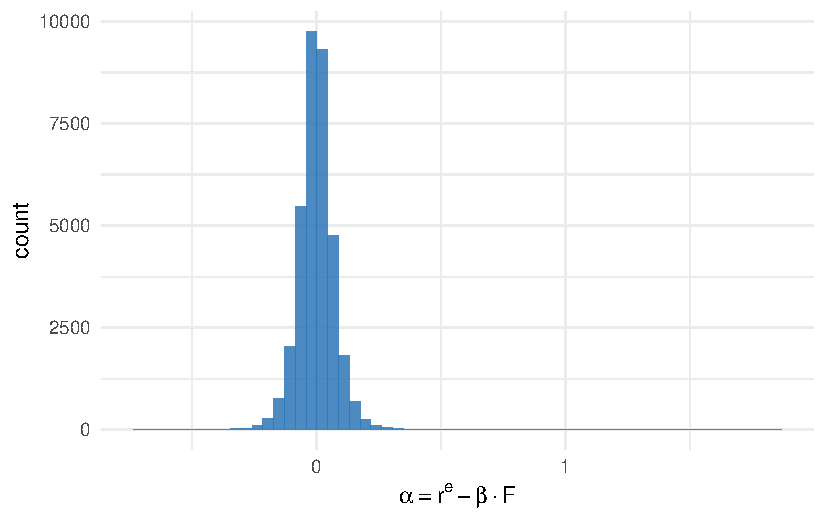
\includegraphics[keepaspectratio]{report_files/figure-pdf/alpha-hist-1.pdf}}

}

\caption{Realised monthly alpha --- symmetric around zero, fat-tailed.}

\end{figure}%

\begin{Shaded}
\begin{Highlighting}[]
\NormalTok{feats }\SpecialCharTok{|\textgreater{}}
  \FunctionTok{filter}\NormalTok{(}\SpecialCharTok{!}\FunctionTok{is.na}\NormalTok{(beta\_mkt)) }\SpecialCharTok{|\textgreater{}}
  \FunctionTok{select}\NormalTok{(beta\_mkt, beta\_smb, beta\_hml, beta\_rmw, beta\_cma) }\SpecialCharTok{|\textgreater{}}
  \FunctionTok{pivot\_longer}\NormalTok{(}\FunctionTok{everything}\NormalTok{(), }\AttributeTok{names\_to =} \StringTok{"factor"}\NormalTok{, }\AttributeTok{values\_to =} \StringTok{"loading"}\NormalTok{) }\SpecialCharTok{|\textgreater{}}
  \FunctionTok{ggplot}\NormalTok{(}\FunctionTok{aes}\NormalTok{(loading)) }\SpecialCharTok{+}
  \FunctionTok{geom\_histogram}\NormalTok{(}\AttributeTok{bins =} \DecValTok{50}\NormalTok{, }\AttributeTok{fill =} \StringTok{"\#1F4E79"}\NormalTok{, }\AttributeTok{alpha =} \FloatTok{0.85}\NormalTok{) }\SpecialCharTok{+}
  \FunctionTok{facet\_wrap}\NormalTok{(}\SpecialCharTok{\textasciitilde{}}\NormalTok{ factor, }\AttributeTok{scales =} \StringTok{"free"}\NormalTok{, }\AttributeTok{ncol =} \DecValTok{5}\NormalTok{) }\SpecialCharTok{+}
  \FunctionTok{labs}\NormalTok{(}\AttributeTok{x =} \ConstantTok{NULL}\NormalTok{, }\AttributeTok{y =} \ConstantTok{NULL}\NormalTok{)}
\end{Highlighting}
\end{Shaded}

\begin{figure}[H]

{\centering \pandocbounded{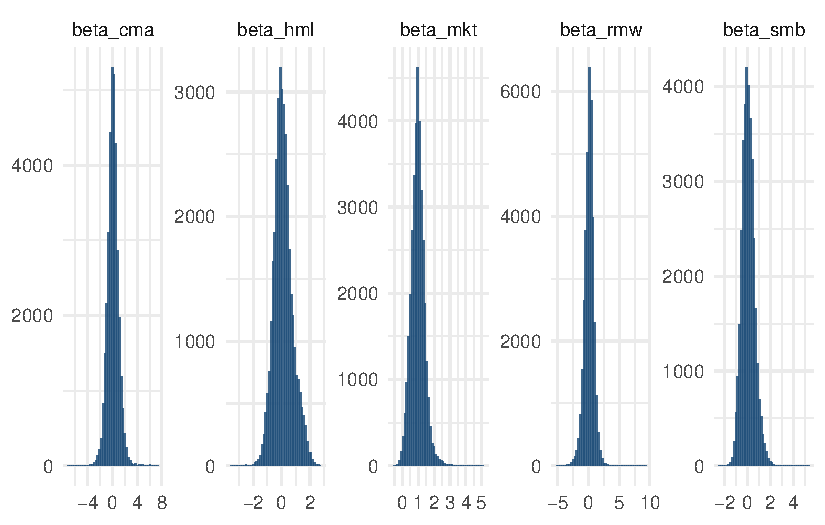
\includegraphics[keepaspectratio]{report_files/figure-pdf/beta-hist-1.pdf}}

}

\caption{FF5 betas across the panel --- mostly market-driven.}

\end{figure}%

\section{5. Clustering on return
co-movement}\label{clustering-on-return-co-movement}

K-Means is fit at the end of each year on the prior sixty months; the
assignment is applied to all twelve months of the following calendar
year.

\begin{Shaded}
\begin{Highlighting}[]
\NormalTok{clust }\OtherTok{\textless{}{-}} \FunctionTok{build\_clusters\_annual}\NormalTok{(panel)}
\end{Highlighting}
\end{Shaded}

\begin{verbatim}
[18:29:20] Building annual K-Means clusters on return co-movement
[18:29:20]   refit 2017-12-31: k=2, sil=0.333, n=325
[18:29:21]   refit 2018-12-31: k=2, sil=0.415, n=339
[18:29:21]   refit 2019-12-31: k=2, sil=0.433, n=358
[18:29:21]   refit 2020-12-31: k=2, sil=0.404, n=379
[18:29:21]   refit 2021-12-31: k=2, sil=0.358, n=391
[18:29:21]   refit 2022-12-31: k=2, sil=0.338, n=409
[18:29:21]   refit 2023-12-31: k=2, sil=0.339, n=421
\end{verbatim}

\begin{Shaded}
\begin{Highlighting}[]
\NormalTok{clust}\SpecialCharTok{$}\NormalTok{diag }\SpecialCharTok{|\textgreater{}}
  \FunctionTok{kable}\NormalTok{(}\AttributeTok{digits =} \DecValTok{3}\NormalTok{, }\AttributeTok{caption =} \StringTok{"Cluster diagnostics by refit date"}\NormalTok{)}
\end{Highlighting}
\end{Shaded}

\begin{longtable}[]{@{}lrrr@{}}
\caption{Cluster diagnostics by refit date}\tabularnewline
\toprule\noalign{}
refit\_date & k & silhouette & n\_stocks \\
\midrule\noalign{}
\endfirsthead
\toprule\noalign{}
refit\_date & k & silhouette & n\_stocks \\
\midrule\noalign{}
\endhead
\bottomrule\noalign{}
\endlastfoot
2017-12-31 & 2 & 0.333 & 325 \\
2018-12-31 & 2 & 0.415 & 339 \\
2019-12-31 & 2 & 0.433 & 358 \\
2020-12-31 & 2 & 0.404 & 379 \\
2021-12-31 & 2 & 0.358 & 391 \\
2022-12-31 & 2 & 0.338 & 409 \\
2023-12-31 & 2 & 0.339 & 421 \\
\end{longtable}

\begin{Shaded}
\begin{Highlighting}[]
\NormalTok{clust}\SpecialCharTok{$}\NormalTok{diag }\SpecialCharTok{|\textgreater{}}
  \FunctionTok{ggplot}\NormalTok{(}\FunctionTok{aes}\NormalTok{(refit\_date, k)) }\SpecialCharTok{+}
  \FunctionTok{geom\_point}\NormalTok{(}\AttributeTok{size =} \FloatTok{2.5}\NormalTok{, }\AttributeTok{colour =} \StringTok{"\#C00000"}\NormalTok{) }\SpecialCharTok{+}
  \FunctionTok{geom\_line}\NormalTok{(}\AttributeTok{colour =} \StringTok{"\#C00000"}\NormalTok{) }\SpecialCharTok{+}
  \FunctionTok{scale\_y\_continuous}\NormalTok{(}\AttributeTok{breaks =} \DecValTok{2}\SpecialCharTok{:}\DecValTok{10}\NormalTok{) }\SpecialCharTok{+}
  \FunctionTok{labs}\NormalTok{(}\AttributeTok{x =} \StringTok{"refit date (end of year)"}\NormalTok{, }\AttributeTok{y =} \StringTok{"chosen k"}\NormalTok{)}
\end{Highlighting}
\end{Shaded}

\begin{figure}[H]

{\centering \pandocbounded{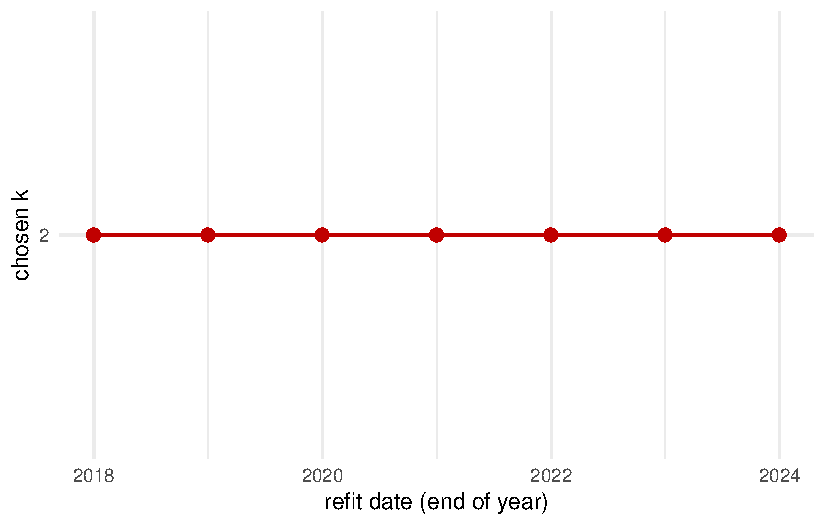
\includegraphics[keepaspectratio]{report_files/figure-pdf/cluster-k-plot-1.pdf}}

}

\caption{Chosen k by refit year. Stability across refits is encouraging
--- drift in \(k\) would suggest the structure is unstable.}

\end{figure}%

\section{6. Three-way comparison}\label{three-way-comparison}

\begin{Shaded}
\begin{Highlighting}[]
\NormalTok{feats\_g }\OtherTok{\textless{}{-}} \FunctionTok{attach\_clusters}\NormalTok{(feats, clust}\SpecialCharTok{$}\NormalTok{assignments)}
\end{Highlighting}
\end{Shaded}

\subsection{6.1 Composition}\label{composition}

How much do the three groupings overlap?

\begin{Shaded}
\begin{Highlighting}[]
\NormalTok{comp }\OtherTok{\textless{}{-}} \FunctionTok{composition\_compare}\NormalTok{(feats\_g)}
\NormalTok{comp}\SpecialCharTok{$}\NormalTok{ari }\SpecialCharTok{|\textgreater{}}
  \FunctionTok{kable}\NormalTok{(}\AttributeTok{digits =} \DecValTok{3}\NormalTok{, }\AttributeTok{caption =} \StringTok{"Adjusted Rand index between scheme pairs"}\NormalTok{)}
\end{Highlighting}
\end{Shaded}

\begin{longtable}[]{@{}lrr@{}}
\caption{Adjusted Rand index between scheme pairs}\tabularnewline
\toprule\noalign{}
comparison & adj\_rand & n\_stocks \\
\midrule\noalign{}
\endfirsthead
\toprule\noalign{}
comparison & adj\_rand & n\_stocks \\
\midrule\noalign{}
\endhead
\bottomrule\noalign{}
\endlastfoot
GICS vs FF12 & 0.464 & 421 \\
GICS vs Cluster & 0.048 & 421 \\
FF12 vs Cluster & 0.033 & 421 \\
\end{longtable}

The adjusted Rand index measures partition similarity, with 1 =
identical and 0 = random. Values close to zero between GICS or FF12 and
the K-Means clusters mean the unsupervised partition is genuinely
different from the industry partitions, which is what we'd want ---
otherwise it adds nothing.

\begin{Shaded}
\begin{Highlighting}[]
\NormalTok{comp}\SpecialCharTok{$}\NormalTok{contingency}\SpecialCharTok{$}\NormalTok{gics\_vs\_cluster }\SpecialCharTok{|\textgreater{}}
  \FunctionTok{as.data.frame.matrix}\NormalTok{() }\SpecialCharTok{|\textgreater{}}
  \FunctionTok{kable}\NormalTok{(}\AttributeTok{caption =} \StringTok{"GICS sector × K{-}Means cluster (most recent month)"}\NormalTok{)}
\end{Highlighting}
\end{Shaded}

\begin{longtable}[]{@{}lrr@{}}
\caption{GICS sector × K-Means cluster (most recent
month)}\tabularnewline
\toprule\noalign{}
& 1 & 2 \\
\midrule\noalign{}
\endfirsthead
\toprule\noalign{}
& 1 & 2 \\
\midrule\noalign{}
\endhead
\bottomrule\noalign{}
\endlastfoot
Communication Services & 7 & 10 \\
Consumer Discretionary & 8 & 34 \\
Consumer Staples & 23 & 9 \\
Energy & 1 & 17 \\
Financials & 9 & 55 \\
Health Care & 35 & 17 \\
Industrials & 9 & 58 \\
Information Technology & 14 & 37 \\
Materials & 3 & 20 \\
Real Estate & 7 & 20 \\
Utilities & 22 & 6 \\
\end{longtable}

\begin{Shaded}
\begin{Highlighting}[]
\NormalTok{comp}\SpecialCharTok{$}\NormalTok{contingency}\SpecialCharTok{$}\NormalTok{ff12\_vs\_cluster }\SpecialCharTok{|\textgreater{}}
  \FunctionTok{as.data.frame.matrix}\NormalTok{() }\SpecialCharTok{|\textgreater{}}
  \FunctionTok{kable}\NormalTok{(}\AttributeTok{caption =} \StringTok{"FF12 industry × K{-}Means cluster (most recent month)"}\NormalTok{)}
\end{Highlighting}
\end{Shaded}

\begin{longtable}[]{@{}lrr@{}}
\caption{FF12 industry × K-Means cluster (most recent
month)}\tabularnewline
\toprule\noalign{}
& 1 & 2 \\
\midrule\noalign{}
\endfirsthead
\toprule\noalign{}
& 1 & 2 \\
\midrule\noalign{}
\endhead
\bottomrule\noalign{}
\endlastfoot
BusEq & 24 & 42 \\
Chems & 5 & 12 \\
Durbl & 1 & 5 \\
Enrgy & 1 & 14 \\
Hlth & 23 & 12 \\
Manuf & 5 & 37 \\
Money & 19 & 66 \\
NoDur & 13 & 11 \\
Other & 7 & 50 \\
Shops & 15 & 20 \\
Telcm & 3 & 6 \\
Utils & 22 & 8 \\
\end{longtable}

\subsection{6.2 Within-group
homogeneity}\label{within-group-homogeneity}

A ``good'' classification produces internally similar members. We
measure this two ways: the cross-sectional standard deviation of
realised alpha within each group at each date (lower = more homogeneous
in unexplained returns), and the mean pairwise correlation of excess
returns among group members (higher = more co-moving).

\begin{Shaded}
\begin{Highlighting}[]
\NormalTok{homo }\OtherTok{\textless{}{-}} \FunctionTok{homogeneity\_compare}\NormalTok{(feats\_g, panel)}
\NormalTok{homo }\SpecialCharTok{|\textgreater{}} \FunctionTok{kable}\NormalTok{(}\AttributeTok{digits =} \DecValTok{4}\NormalTok{, }\AttributeTok{caption =} \StringTok{"Within{-}group homogeneity by scheme"}\NormalTok{)}
\end{Highlighting}
\end{Shaded}

\begin{longtable}[]{@{}
  >{\raggedright\arraybackslash}p{(\linewidth - 8\tabcolsep) * \real{0.1081}}
  >{\raggedleft\arraybackslash}p{(\linewidth - 8\tabcolsep) * \real{0.1892}}
  >{\raggedleft\arraybackslash}p{(\linewidth - 8\tabcolsep) * \real{0.2162}}
  >{\raggedleft\arraybackslash}p{(\linewidth - 8\tabcolsep) * \real{0.2297}}
  >{\raggedleft\arraybackslash}p{(\linewidth - 8\tabcolsep) * \real{0.2568}}@{}}
\caption{Within-group homogeneity by scheme}\tabularnewline
\toprule\noalign{}
\begin{minipage}[b]{\linewidth}\raggedright
scheme
\end{minipage} & \begin{minipage}[b]{\linewidth}\raggedleft
mean\_alpha\_sd
\end{minipage} & \begin{minipage}[b]{\linewidth}\raggedleft
median\_alpha\_sd
\end{minipage} & \begin{minipage}[b]{\linewidth}\raggedleft
mean\_within\_corr
\end{minipage} & \begin{minipage}[b]{\linewidth}\raggedleft
median\_within\_corr
\end{minipage} \\
\midrule\noalign{}
\endfirsthead
\toprule\noalign{}
\begin{minipage}[b]{\linewidth}\raggedright
scheme
\end{minipage} & \begin{minipage}[b]{\linewidth}\raggedleft
mean\_alpha\_sd
\end{minipage} & \begin{minipage}[b]{\linewidth}\raggedleft
median\_alpha\_sd
\end{minipage} & \begin{minipage}[b]{\linewidth}\raggedleft
mean\_within\_corr
\end{minipage} & \begin{minipage}[b]{\linewidth}\raggedleft
median\_within\_corr
\end{minipage} \\
\midrule\noalign{}
\endhead
\bottomrule\noalign{}
\endlastfoot
GICS & 0.0626 & 0.0587 & 0.4710 & 0.4505 \\
FF12 & 0.0638 & 0.0599 & 0.4525 & 0.4432 \\
Cluster & 0.0679 & 0.0642 & 0.3366 & 0.3366 \\
\end{longtable}

If the K-Means scheme is doing its job, it should win on
\texttt{mean\_within\_corr} --- that's what it was optimised for. The
question is whether GICS or FF12 closes that gap.

\subsection{6.3 Predictive accuracy}\label{predictive-accuracy}

Per-group Elastic Net regressions predict \(\alpha_{i,t+1}\) from the
feature set. We report out-of-sample R², MAE, and directional accuracy
on the 2023--2024 holdout, weighted by group size.

\begin{Shaded}
\begin{Highlighting}[]
\NormalTok{pred }\OtherTok{\textless{}{-}} \FunctionTok{prediction\_compare}\NormalTok{(feats\_g)}
\end{Highlighting}
\end{Shaded}

\begin{verbatim}
[18:29:22] Prediction: train n=7281, test n=3336
\end{verbatim}

\begin{Shaded}
\begin{Highlighting}[]
\NormalTok{pred}\SpecialCharTok{$}\NormalTok{aggregate }\SpecialCharTok{|\textgreater{}}
  \FunctionTok{arrange}\NormalTok{(}\FunctionTok{desc}\NormalTok{(r2\_oos\_weighted)) }\SpecialCharTok{|\textgreater{}}
  \FunctionTok{kable}\NormalTok{(}\AttributeTok{digits =} \DecValTok{4}\NormalTok{, }\AttributeTok{caption =} \StringTok{"Aggregate prediction metrics by scheme"}\NormalTok{)}
\end{Highlighting}
\end{Shaded}

\begin{longtable}[]{@{}
  >{\raggedright\arraybackslash}p{(\linewidth - 10\tabcolsep) * \real{0.1053}}
  >{\raggedleft\arraybackslash}p{(\linewidth - 10\tabcolsep) * \real{0.1711}}
  >{\raggedleft\arraybackslash}p{(\linewidth - 10\tabcolsep) * \real{0.2105}}
  >{\raggedleft\arraybackslash}p{(\linewidth - 10\tabcolsep) * \real{0.1711}}
  >{\raggedleft\arraybackslash}p{(\linewidth - 10\tabcolsep) * \real{0.2237}}
  >{\raggedleft\arraybackslash}p{(\linewidth - 10\tabcolsep) * \real{0.1184}}@{}}
\caption{Aggregate prediction metrics by scheme}\tabularnewline
\toprule\noalign{}
\begin{minipage}[b]{\linewidth}\raggedright
scheme
\end{minipage} & \begin{minipage}[b]{\linewidth}\raggedleft
n\_test\_total
\end{minipage} & \begin{minipage}[b]{\linewidth}\raggedleft
r2\_oos\_weighted
\end{minipage} & \begin{minipage}[b]{\linewidth}\raggedleft
mae\_weighted
\end{minipage} & \begin{minipage}[b]{\linewidth}\raggedleft
dir\_acc\_weighted
\end{minipage} & \begin{minipage}[b]{\linewidth}\raggedleft
n\_groups
\end{minipage} \\
\midrule\noalign{}
\endfirsthead
\toprule\noalign{}
\begin{minipage}[b]{\linewidth}\raggedright
scheme
\end{minipage} & \begin{minipage}[b]{\linewidth}\raggedleft
n\_test\_total
\end{minipage} & \begin{minipage}[b]{\linewidth}\raggedleft
r2\_oos\_weighted
\end{minipage} & \begin{minipage}[b]{\linewidth}\raggedleft
mae\_weighted
\end{minipage} & \begin{minipage}[b]{\linewidth}\raggedleft
dir\_acc\_weighted
\end{minipage} & \begin{minipage}[b]{\linewidth}\raggedleft
n\_groups
\end{minipage} \\
\midrule\noalign{}
\endhead
\bottomrule\noalign{}
\endlastfoot
Cluster & 3302 & -0.0844 & 0.0562 & 0.4761 & 2 \\
Pooled & 3336 & -0.0936 & 0.0567 & 0.4661 & 1 \\
GICS & 3336 & -0.2813 & 0.0619 & 0.4865 & 11 \\
FF12 & 3336 & -0.4075 & 0.0649 & 0.4766 & 12 \\
\end{longtable}

\begin{Shaded}
\begin{Highlighting}[]
\NormalTok{pred}\SpecialCharTok{$}\NormalTok{per\_group }\SpecialCharTok{|\textgreater{}}
  \FunctionTok{ggplot}\NormalTok{(}\FunctionTok{aes}\NormalTok{(}\FunctionTok{reorder}\NormalTok{(group, r2\_oos), r2\_oos, }\AttributeTok{fill =}\NormalTok{ scheme)) }\SpecialCharTok{+}
  \FunctionTok{geom\_col}\NormalTok{() }\SpecialCharTok{+}
  \FunctionTok{coord\_flip}\NormalTok{() }\SpecialCharTok{+}
  \FunctionTok{facet\_wrap}\NormalTok{(}\SpecialCharTok{\textasciitilde{}}\NormalTok{ scheme, }\AttributeTok{scales =} \StringTok{"free\_y"}\NormalTok{) }\SpecialCharTok{+}
  \FunctionTok{labs}\NormalTok{(}\AttributeTok{x =} \ConstantTok{NULL}\NormalTok{, }\AttributeTok{y =} \StringTok{"out{-}of{-}sample R²"}\NormalTok{, }\AttributeTok{fill =} \ConstantTok{NULL}\NormalTok{,}
       \AttributeTok{title =} \StringTok{"OOS R² per group, by scheme"}\NormalTok{) }\SpecialCharTok{+}
  \FunctionTok{scale\_fill\_manual}\NormalTok{(}\AttributeTok{values =} \FunctionTok{c}\NormalTok{(}\AttributeTok{GICS =} \StringTok{"\#1F4E79"}\NormalTok{, }\AttributeTok{FF12 =} \StringTok{"\#2E75B6"}\NormalTok{, }\AttributeTok{Cluster =} \StringTok{"\#C00000"}\NormalTok{)) }\SpecialCharTok{+}
  \FunctionTok{theme}\NormalTok{(}\AttributeTok{legend.position =} \StringTok{"none"}\NormalTok{)}
\end{Highlighting}
\end{Shaded}

\pandocbounded{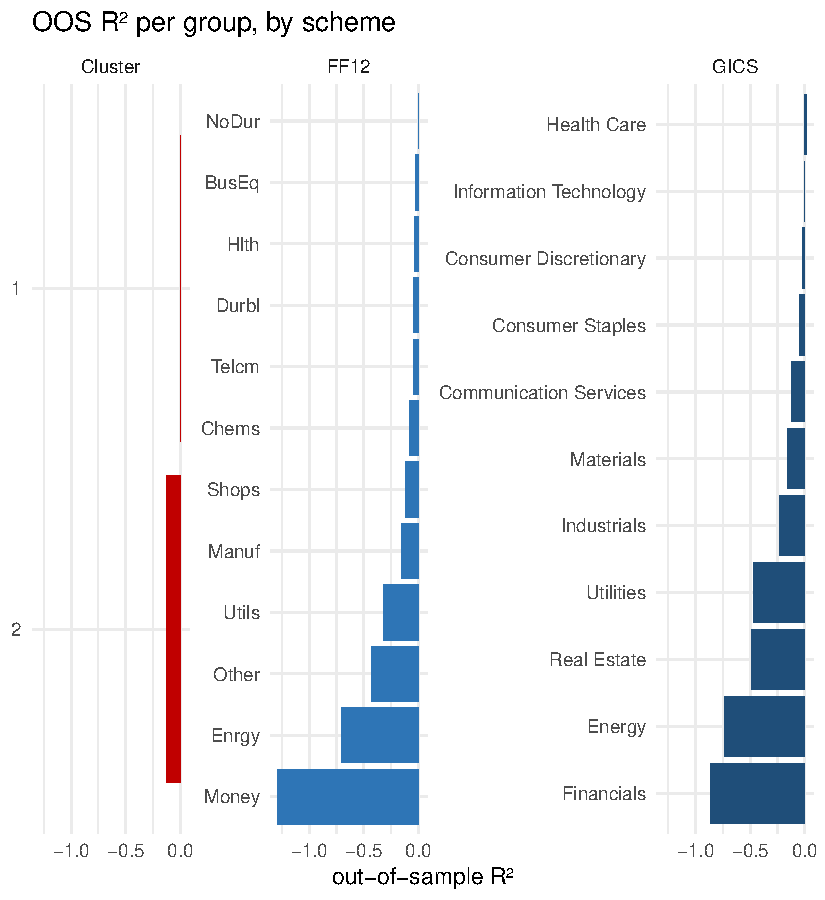
\includegraphics[keepaspectratio]{report_files/figure-pdf/prediction-per-group-1.pdf}}

The pooled baseline (no grouping) gives a single all-stocks Elastic Net.
If any of the three schemes can beat the pooled model on R² \emph{and}
directional accuracy, that scheme is adding information beyond what the
features carry on their own.

\subsection{6.4 Anomaly detection}\label{anomaly-detection}

Isolation Forest is trained per group on the train window and scored on
the holdout; the most anomalous five percent are flagged. We then look
at average forward alpha at one, three, and six months for flagged
versus non-flagged stocks.

\begin{Shaded}
\begin{Highlighting}[]
\NormalTok{anom }\OtherTok{\textless{}{-}} \FunctionTok{anomaly\_compare}\NormalTok{(feats\_g)}
\end{Highlighting}
\end{Shaded}

\begin{verbatim}
[18:29:23]   iForest within GICS
[18:29:23]   iForest within FF12
[18:29:23]   iForest within Cluster
\end{verbatim}

\begin{Shaded}
\begin{Highlighting}[]
\NormalTok{anom}\SpecialCharTok{$}\NormalTok{fwd\_compare }\SpecialCharTok{|\textgreater{}}
  \FunctionTok{arrange}\NormalTok{(scheme, horizon, flagged) }\SpecialCharTok{|\textgreater{}}
  \FunctionTok{kable}\NormalTok{(}\AttributeTok{digits =} \DecValTok{4}\NormalTok{,}
        \AttributeTok{caption =} \StringTok{"Mean forward alpha for flagged vs. non{-}flagged stocks, by scheme and horizon"}\NormalTok{)}
\end{Highlighting}
\end{Shaded}

\begin{longtable}[]{@{}llrrrr@{}}
\caption{Mean forward alpha for flagged vs.~non-flagged stocks, by
scheme and horizon}\tabularnewline
\toprule\noalign{}
scheme & flagged & horizon & n & mean\_fwd\_alpha &
median\_fwd\_alpha \\
\midrule\noalign{}
\endfirsthead
\toprule\noalign{}
scheme & flagged & horizon & n & mean\_fwd\_alpha &
median\_fwd\_alpha \\
\midrule\noalign{}
\endhead
\bottomrule\noalign{}
\endlastfoot
Cluster & FALSE & 1 & 3135 & -0.0050 & -0.0053 \\
Cluster & TRUE & 1 & 167 & -0.0149 & -0.0082 \\
Cluster & FALSE & 3 & 2737 & -0.0031 & -0.0028 \\
Cluster & TRUE & 3 & 161 & 0.0054 & 0.0104 \\
Cluster & FALSE & 6 & 2327 & -0.0028 & -0.0018 \\
Cluster & TRUE & 6 & 150 & -0.0129 & -0.0062 \\
FF12 & FALSE & 1 & 3164 & -0.0054 & -0.0048 \\
FF12 & TRUE & 1 & 172 & -0.0096 & -0.0143 \\
FF12 & FALSE & 3 & 2762 & -0.0030 & -0.0023 \\
FF12 & TRUE & 3 & 162 & -0.0017 & -0.0017 \\
FF12 & FALSE & 6 & 2355 & -0.0030 & -0.0018 \\
FF12 & TRUE & 6 & 143 & -0.0091 & -0.0058 \\
GICS & FALSE & 1 & 3163 & -0.0048 & -0.0047 \\
GICS & TRUE & 1 & 173 & -0.0207 & -0.0151 \\
GICS & FALSE & 3 & 2761 & -0.0026 & -0.0021 \\
GICS & TRUE & 3 & 163 & -0.0082 & -0.0084 \\
GICS & FALSE & 6 & 2352 & -0.0031 & -0.0019 \\
GICS & TRUE & 6 & 146 & -0.0089 & -0.0051 \\
\end{longtable}

\begin{Shaded}
\begin{Highlighting}[]
\NormalTok{anom}\SpecialCharTok{$}\NormalTok{fwd\_compare }\SpecialCharTok{|\textgreater{}}
  \FunctionTok{group\_by}\NormalTok{(scheme, horizon) }\SpecialCharTok{|\textgreater{}}
  \FunctionTok{summarise}\NormalTok{(}
    \AttributeTok{gap =}\NormalTok{ mean\_fwd\_alpha[flagged] }\SpecialCharTok{{-}}\NormalTok{ mean\_fwd\_alpha[}\SpecialCharTok{!}\NormalTok{flagged],}
    \AttributeTok{.groups =} \StringTok{"drop"}
\NormalTok{  ) }\SpecialCharTok{|\textgreater{}}
  \FunctionTok{ggplot}\NormalTok{(}\FunctionTok{aes}\NormalTok{(}\FunctionTok{factor}\NormalTok{(horizon), gap, }\AttributeTok{fill =}\NormalTok{ scheme)) }\SpecialCharTok{+}
  \FunctionTok{geom\_col}\NormalTok{(}\AttributeTok{position =} \FunctionTok{position\_dodge}\NormalTok{(}\AttributeTok{width =} \FloatTok{0.8}\NormalTok{), }\AttributeTok{width =} \FloatTok{0.7}\NormalTok{) }\SpecialCharTok{+}
  \FunctionTok{geom\_hline}\NormalTok{(}\AttributeTok{yintercept =} \DecValTok{0}\NormalTok{) }\SpecialCharTok{+}
  \FunctionTok{scale\_fill\_manual}\NormalTok{(}\AttributeTok{values =} \FunctionTok{c}\NormalTok{(}\AttributeTok{GICS =} \StringTok{"\#1F4E79"}\NormalTok{, }\AttributeTok{FF12 =} \StringTok{"\#2E75B6"}\NormalTok{, }\AttributeTok{Cluster =} \StringTok{"\#C00000"}\NormalTok{)) }\SpecialCharTok{+}
  \FunctionTok{labs}\NormalTok{(}\AttributeTok{x =} \StringTok{"horizon (months ahead)"}\NormalTok{,}
       \AttributeTok{y =} \StringTok{"mean forward alpha (flagged − non{-}flagged)"}\NormalTok{, }\AttributeTok{fill =} \ConstantTok{NULL}\NormalTok{)}
\end{Highlighting}
\end{Shaded}

\begin{figure}[H]

{\centering \pandocbounded{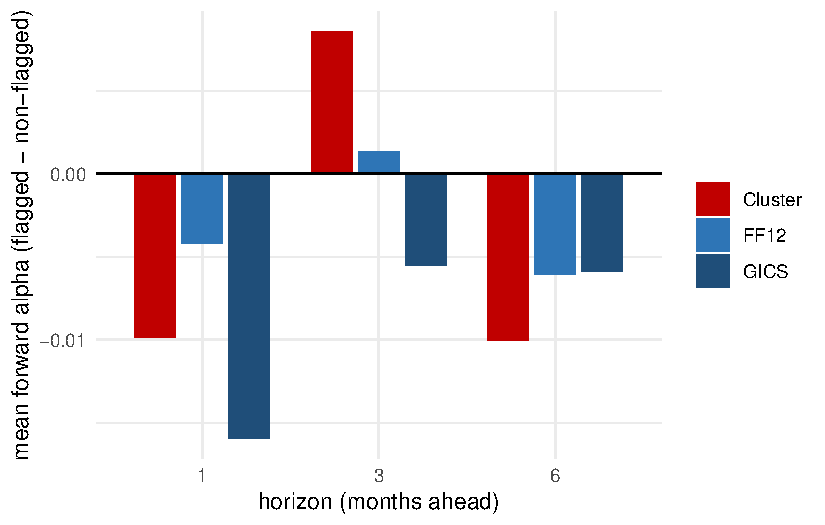
\includegraphics[keepaspectratio]{report_files/figure-pdf/anomaly-fwd-plot-1.pdf}}

}

\caption{Forward alpha gap (flagged minus non-flagged) by horizon. A
negative bar at +1m would suggest flagged stocks subsequently
underperform on a risk-adjusted basis --- the mispricing reading.}

\end{figure}%

\begin{Shaded}
\begin{Highlighting}[]
\NormalTok{anom}\SpecialCharTok{$}\NormalTok{flag\_overlap }\SpecialCharTok{|\textgreater{}}
  \FunctionTok{filter}\NormalTok{(a }\SpecialCharTok{!=}\NormalTok{ b) }\SpecialCharTok{|\textgreater{}}
  \FunctionTok{kable}\NormalTok{(}\AttributeTok{digits =} \DecValTok{3}\NormalTok{,}
        \AttributeTok{caption =} \StringTok{"Pairwise Jaccard overlap of flagged (permno, date\_eom) keys"}\NormalTok{)}
\end{Highlighting}
\end{Shaded}

\begin{longtable}[]{@{}llrrr@{}}
\caption{Pairwise Jaccard overlap of flagged (permno, date\_eom)
keys}\tabularnewline
\toprule\noalign{}
a & b & n\_a & n\_b & jaccard \\
\midrule\noalign{}
\endfirsthead
\toprule\noalign{}
a & b & n\_a & n\_b & jaccard \\
\midrule\noalign{}
\endhead
\bottomrule\noalign{}
\endlastfoot
GICS & FF12 & 173 & 172 & 0.426 \\
GICS & Cluster & 173 & 167 & 0.344 \\
FF12 & GICS & 172 & 173 & 0.426 \\
FF12 & Cluster & 172 & 167 & 0.351 \\
Cluster & GICS & 167 & 173 & 0.344 \\
Cluster & FF12 & 167 & 172 & 0.351 \\
\end{longtable}

\section{7. Discussion}\label{discussion}

The four-dimensional comparison gives a more complete answer than any
single metric:

\begin{itemize}
\tightlist
\item
  \textbf{Composition.} Low Rand-index values between K-Means and either
  of the industry schemes confirm that the unsupervised clustering finds
  structure that is not reducible to industry codes. The GICS-FF12 ARI
  is expected to be the highest of the three pairs --- both partitions
  are ultimately built around the same notion of what a firm ``does.''
\item
  \textbf{Homogeneity.} Co-movement clusters are constructed to maximise
  within-group return correlation, so they should win on
  \texttt{mean\_within\_corr} by design. The interesting question is
  whether GICS or FF12 produces lower alpha-dispersion within groups ---
  that would indicate that industry membership \emph{also} organises
  unexplained-return behaviour, even though the schemes were not built
  with alpha in mind.
\item
  \textbf{Prediction.} The economically meaningful comparison is whether
  per-group models beat the pooled baseline. If they do, the grouping is
  carrying information that conditions the alpha-forecasting
  relationship --- different industries respond differently to factor
  exposures and macro conditions. If the pooled model wins, the data is
  telling us there isn't enough sample within any single industry or
  cluster to reliably estimate group-specific dynamics, and one global
  model is the right answer.
\item
  \textbf{Anomalies.} A scheme whose Isolation Forest flags subsequently
  earn meaningfully different forward alpha --- and where that
  difference persists at 3 and 6 months rather than mean-reverting in a
  single month --- has a credible mispricing reading. If all three
  schemes flag similar-quality anomalies, the choice of grouping doesn't
  matter much for outlier detection, and one would prefer the simpler /
  more interpretable scheme (GICS).
\end{itemize}

Two caveats. First, the dev-mode subset of fifty stocks limits how much
weight the numbers can bear; a full S\&P 500 run is necessary before
treating these comparisons as decisive. Second, the alpha computation is
itself dependent on the FF5 specification --- alpha that the FF5 model
fails to absorb might still be priced by extensions (momentum, quality,
short-term reversal). Our anomaly definition is ``FF5-residual,'' not
``genuinely unexplained.''

\section{8. Limitations and next
steps}\label{limitations-and-next-steps}

\begin{itemize}
\tightlist
\item
  \textbf{Universe size.} Final numbers should come from
  \texttt{CFG\$dev\_mode\ =\ FALSE} on the full universe, not the
  50-stock sample.
\item
  \textbf{Cluster stability.} The annual-refit + Hungarian-matching
  pipeline keeps cluster IDs stable but doesn't guarantee that the
  underlying groupings are stable. A robustness check that varies the
  refit window (say, 36 vs.~60 vs.~84 months) would be useful.
\item
  \textbf{Alternative anomaly horizons.} Six months is the longest
  forward horizon we report. Some mispricing-reversion stories play out
  over a year or longer; extending the horizon would test those.
\item
  \textbf{Sector-conditional clustering.} A natural follow-up is K-Means
  \emph{within} GICS sectors --- does sub-sectoral clustering find
  structure that flat clustering misses?
\end{itemize}

\section{Outputs}\label{outputs}

\begin{Shaded}
\begin{Highlighting}[]
\FunctionTok{list.files}\NormalTok{(}\FunctionTok{c}\NormalTok{(PATHS}\SpecialCharTok{$}\NormalTok{raw, PATHS}\SpecialCharTok{$}\NormalTok{processed),}
           \AttributeTok{pattern =} \StringTok{"}\SpecialCharTok{\textbackslash{}\textbackslash{}}\StringTok{.parquet$"}\NormalTok{, }\AttributeTok{full.names =} \ConstantTok{TRUE}\NormalTok{) }\SpecialCharTok{|\textgreater{}}
  \FunctionTok{tibble}\NormalTok{(}\AttributeTok{file =}\NormalTok{ \_) }\SpecialCharTok{|\textgreater{}}
  \FunctionTok{mutate}\NormalTok{(}\AttributeTok{size\_kb =} \FunctionTok{round}\NormalTok{(}\FunctionTok{file.size}\NormalTok{(file) }\SpecialCharTok{/} \DecValTok{1024}\NormalTok{, }\DecValTok{1}\NormalTok{)) }\SpecialCharTok{|\textgreater{}}
  \FunctionTok{kable}\NormalTok{()}
\end{Highlighting}
\end{Shaded}

{\def\LTcaptype{none} % do not increment counter
\begin{longtable}[]{@{}lr@{}}
\toprule\noalign{}
file & size\_kb \\
\midrule\noalign{}
\endhead
\bottomrule\noalign{}
\endlastfoot
data/processed/clusters\_annual.parquet & 25.0 \\
data/processed/clusters\_diag.parquet & 1.4 \\
data/processed/features.parquet & 7273.9 \\
data/processed/panel.parquet & 1214.6 \\
data/raw/ccm\_gics.parquet & 13.6 \\
data/raw/crsp\_msf.parquet & 1106.8 \\
data/raw/crsp\_sic\_history.parquet & 6.3 \\
data/raw/crsp\_stocknames.parquet & 17.9 \\
data/raw/ff12\_def.parquet & 3.0 \\
data/raw/ff5.parquet & 26.6 \\
data/raw/fred\_dff.parquet & 184.1 \\
data/raw/fred\_dgs10.parquet & 125.3 \\
data/raw/fred\_vixcls.parquet & 79.0 \\
data/raw/sp500\_members.parquet & 9.6 \\
\end{longtable}
}




\end{document}
